\subsection{Overview}

In the field of Information Retrieval [NOTE], there are techniques being widely used in several applications. They can be considered as a basic and indispensable part of a knowledge mining system. [AGGIUNGERE QUALCOSA]

\subsection{Mathematical Background}

%%%%%%%%%%%%%%%%%%%%%%%%%%%%%%%%%%%%%%%%%%%%%%%%%%%%%%%%%%

\subsubsection{Term-Document Matrix}
 In Natural Language Processing \cite{Collobert:2011:NLP:1953048.2078186}, a term-document matrix (TDM) is used to represent the relationships between words and documents \cite{Turney:2010:FMV:1861751.1861756}. In a TDM, each row corresponds to a document and each column corresponds to a term. A cell in the TDM represents the weight of a term in a document. The most common weighting scheme used in document retrieval is the \emph{term frequency-inverse document frequency (tf-idf)} function \cite{Reed:2006:TNT:1193211.1193734}. If we consider a set of $n$ documents $D=(d_{1},d_{2},..,d_{n})$ and a set of terms $t=(t_{1},t_{2},..,t_{r})$ then the representation of a document $d \in D $ is vector $\vec{\delta}=(w_{1}^{d},w_{2}^{d},..,w_{r}^{d})$, where the weight $w_{k}^{d}$ of term $k$ in document $d$ is computed using the {\em tf-idf} function \cite{Ramos1999}:

\begin{equation} \label{tfidf} %\nonumber 
w_{k}^{d} =tf\cdot idf(k,d,D)= f_{k}^{d}\cdot log\frac{n}{\left | \left \{ d\in D: t_{k} \in d \right \} \right |} 
\end{equation}

where $f_{k}^{d}$ is the frequency of term $t_{k}$ in document $d$.

Another common weighting scheme uses only the frequency of terms in documents for cells in TDM, i.e. the number of occurrence of a term in a document, instead of {\em tf-idf}. As an example, we consider a set of three simple documents $D=(d_{1},d_{2},d_{3})$ as follows:

\begin{itemize}
	\item[+] $d_{1}$: \emph{She is nice.}
	\item[+] $d_{2}$: \emph{Today is nice.}
	\item[+] $d_{3}$: \emph{Nice is a nice city.}
\end{itemize}

\begin{figure}[h!]
	\begin{equation} \nonumber
	\bordermatrix{~ & she & is & today & a & nice & city \cr	
		d_{1} 		& 1 & 1 & 0 & 0 & 1 & 0 \cr 
		d_{2} 		& 0 & 1 & 1 & 0 & 1 & 0 \cr  
		d_{3} 		& 0 & 1 & 0 & 1 & 2 & 1 \cr }
	\end{equation}
	\caption{An example of a term-document matrix}
	\label{fig:TDM}
\end{figure}

The set of terms $t$ consists of $6$ elements, i.e. $t=(she$, $is$, $today$, $a$, $nice$, $city)$ and the corresponding term-document matrix for $D$ is depicted in Figure \ref{fig:TDM}.

TDM has been exploited to characterize software systems and finally to compute similarities between them \cite{10.1109/APSEC.2004.69},\cite{10.1109ICPC.2016.7503721},\cite{McMillan:2012:DSS:2337223.2337267}. In a TDM for software systems, each row represents a package, an API call or a function and each column represents a software system. A cell in the matrix is the number of occurrence of a package/an API/function in each corresponding software system. A TDM for software systems has a similar form to the matrix shown in Figure \ref{fig:TDM} where documents are replaced by software systems and terms are replaced by API calls.

%%%%%%%%%%%%%%%%%%%%%%%%%%%%%%%%%%%%%%%%%%%%%%%%%%%%%%%%%%

\subsubsection{Cosine Similarity}

Cosine similarity is a metric used to compute similarity between two objects using their feature vectors \cite{tversky1977features}. An object is characterized as a vector, and for a pair of vectors $\vec{\alpha}=(\alpha_{1},\alpha_{2},..,\alpha_{n})$ and $\vec{\beta}=(\beta_{1},\beta_{2},..,\beta_{n})$ there is an angle between them. Intuitively, the cosine similarity metric measures the similarity as the cosine of the corresponding angle between the two vectors and it is computed using the inner product as follows. 

\begin{equation} \label{eqn:Cosine}
CosineSim(\vec{\alpha},\vec{\beta}) = \frac{\sum_{i=1}^{n}\alpha_{i}\cdot \beta_{i}}{\sqrt{\sum_{i=1}^{n}(\alpha_{i})^{2} }\cdot \sqrt{\sum_{i=1}^{n}(\beta_{i})^{2}}}
\end{equation}

Figure \ref{fig:Cosine} illustrates the cosine similarity between two vectors $\vec{\alpha}$ and $\vec{\beta}$ in a three-dimension space. This can be thought as the similarity between two documents with three terms $t=(t_{1},t_{2},t_{3})$.

\begin{figure}[h!]
	\centering
	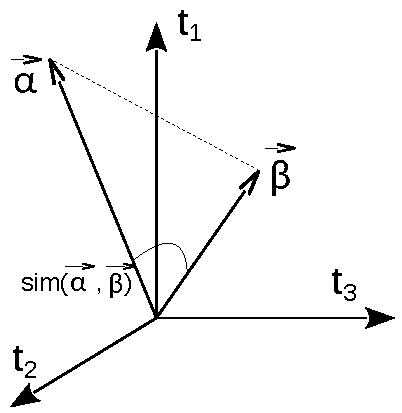
\includegraphics[width=0.25\textwidth]{images/Cosine.pdf}
	\caption{Cosine similarity between two feature vectors $\vec{\alpha}$ and $\vec{\beta}$}
	\label{fig:Cosine}
\end{figure}

Cosine similarity has been popularly adopted in many applications that are related to similarity measurement in various domains \cite{Huang:2012:LCD:2343876.2343884},\cite{Islam:2008:STS:1376815.1376819},\cite{Linden:2003:ARI:642462.642471},\cite{conf:iscis:MadylovaO09},\cite{Mihalcea:2006:CKM:1597538.1597662}. Among the similarity metrics being recalled in this deliverable, the prevalence of Cosine Similarity is obvious as it is utilized in almost all of them as follows: \textit{MUDABlue} \cite{10.1109/APSEC.2004.69}, \textit{CLAN} \cite{McMillan:2012:DSS:2337223.2337267}, \textit{CLANdroid} \cite{10.1109ICPC.2016.7503721}, \textit{LibRec} \cite{6671293}, \textit{SimApp} \cite{Chen:2015:SFD:2684822.2685305}, \textit{WuKong} \cite{Wang:2015:WSA:2771783.2771795}, \textit{TagSim} \cite{Lo:2012:DSA:2473496.2473616}, and \textit{RepoPal} \cite{10.1109/SANER.2017.7884605}

%%%%%%%%%%%%%%%%%%%%%%%%%%%%%%%%%%%%%%%%%%%%%%%%%%%%%%%%%%  

\subsubsection{Latent Semantic Analysis}

The problem with the term-document matrix is that the intrinsic relationships among different terms of a document cannot fully be captured. Furthermore, same words can be used to explain different requirements or the other way around, the same requirements can be described using different words \cite{10.1109/APSEC.2004.69}. Latent Semantic Analysis (LSA), also known as Latent Semantic Indexing (LSI), has been proposed to overcome these problems \cite{Landauer1998}. The technique exploits a mathematical model that can infer latent semantic relationships to compute similarity. LSA represents the contextual usage meaning of words by statistical computations applied to a large corpus of text. It then generates a representation that captures the similarity of words and text passages. To perform LSA on a text, a term-document matrix is created to characterize the text. Afterwards, Singular Value Decomposition (SVD) - a matrix decomposition technique - is used in combination with LSA to reduce matrix dimensionality \cite{kb2005}. SVD takes a highly variable set of data entries as input and transforms to a lower dimensional space but reveals the substructure of the original data. Essentially, it decomposes a rectangular matrix into the product of three other matrices as given below\cite{kb2005}:

\begin{equation}
A_{mn}=U_{mm}S_{mn}V_{mn}^{T}
\end{equation}

in which

\begin{itemize}
	\item $U_{mm}$: Orthogonal matrix.
	\item $S_{mn}$: Diagonal matrix.
	\item $V_{mn}^{T}$: The transpose of an orthogonal matrix.
	\item $X$: Low Rank matrix.
\end{itemize}


$U_{mm}$ describes the original row entities as vectors of derived orthogonal factor values. $S_{mn}$ represents the original column entities in the same way, and $V_{mn}$ is a diagonal matrix containing scaling values. With the application of LSA it is possible to find the most relevant features and remove the least important ones by means of the reduced matrix $U_{mm}$. As a result, an equivalence of $A_{mm}$ can be constructed using the most relevant features. LSA helps reveal the latent relationship among words as well as among passages which cannot be guaranteed by a simple term-document matrix. The similarity measurement by LSA reflects adequately human perception of similarity and association among texts. Using LSA, similarities among documents are measured as the cosine of the angle between their row vectors (see Sec. \ref{sec:cosine}). LSA has been applied in \cite{10.1109/APSEC.2004.69},\cite{10.1109ICPC.2016.7503721},\cite{McMillan:2012:DSS:2337223.2337267} to compute similarities of software systems. The main disadvantage of LSA is that it is computational expensive when a large amount of information is analyzed.
Another very relevant issue related to LSA is the low rank approximation applied by the SVD procedure. If the singular values in $S_{mn}$ are ordered by size, the first k largest may be kept and the remaining smaller ones set to zero. The product of the resulting matrices is a matrix $X$ which is only approximately equal to $A_{mm}$ , and is of rank k . It can be shown that the new matrix $X$ is the matrix of rank k which is closest in the least squares sense to $A_{mm}$ .
The amount of dimension reduction, i.e., the choice of k , is critical to our work. Ideally, we want a value of k that is large enough to fit all the real structure in the data, but small enough so that we do not also fit the sampling error or unimportant details. The proper way to make such choices is an open issue in the factor analytic literature. In practice, we currently use an operational criterion - a
value of k which yields good retrieval performance. In our we decided a k value = numer of reposotories/2 [TO BE COMPLETED]